\documentclass[letterpaper,journal]{IEEEtran}
\usepackage{amsmath,amssymb,amsfonts,amsthm,graphicx,booktabs,xcolor}
\usepackage{xr}
\usepackage{url}
\newcommand{\cref}[1]{Proposition~\ref{#1}}
% import labels from the main paper, but not its citation numbers (the supplement has its own bibliography)
\makeatletter\begingroup\let\bibcite\@gobbletwo\externaldocument{main}\endgroup\makeatother
\newcommand{\LoneHard}{46.6}
\newcommand{\LoneLam}{0.50}
\newcommand{\LoneRone}{59.9}
\newcommand{\LtenHard}{47.7}
\newcommand{\LtenLam}{0.50}
\newcommand{\LtenRone}{60.7}
\newcommand{\famFrGal}{59.5}
\newcommand{\famFrGalVsHalfHi}{+0.7}
\newcommand{\famFrGalVsHalfLo}{-0.3}
\newcommand{\famFrGalVsHalfMean}{+0.2}
\newcommand{\famFrGalVsSalHi}{+0.9}
\newcommand{\famFrGalVsSalLo}{-0.9}
\newcommand{\famFrGalVsSalMean}{-0.1}
\newcommand{\famFrGalsd}{1.3}
\newcommand{\famFrLamH}{59.4}
\newcommand{\famFrLamHsd}{0.9}
\newcommand{\famFrLamQ}{60.0}
\newcommand{\famFrLamQsd}{1.1}
\newcommand{\famFrLamRange}{1.5}
\newcommand{\famFrLamTQ}{58.6}
\newcommand{\famFrLamTQsd}{1.0}
\newcommand{\famFrLamZero}{60.1}
\newcommand{\famFrLamZeroND}{60.3}
\newcommand{\famFrLamZeroNDsd}{1.0}
\newcommand{\famFrLamZerosd}{0.9}
\newcommand{\famFrNDvsDHi}{+0.7}
\newcommand{\famFrNDvsDLo}{-0.5}
\newcommand{\famFrNDvsDMean}{+0.1}
\newcommand{\famFrNv}{57.8}
\newcommand{\famFrNvVsNDHi}{-1.2}
\newcommand{\famFrNvVsNDLo}{-3.7}
\newcommand{\famFrNvVsNDMean}{-2.4}
\newcommand{\famFrNvsd}{0.7}
\newcommand{\famFrSal}{59.6}
\newcommand{\famFrSalND}{55.8}
\newcommand{\famFrSalNDsd}{1.5}
\newcommand{\famFrSalNDvsDHi}{-2.7}
\newcommand{\famFrSalNDvsDLo}{-4.8}
\newcommand{\famFrSalNDvsDMean}{-3.8}
\newcommand{\famFrSalsd}{0.4}
\newcommand{\famFtGal}{71.3}
\newcommand{\famFtGalVsHalfHi}{+0.3}
\newcommand{\famFtGalVsHalfLo}{-1.6}
\newcommand{\famFtGalVsHalfMean}{-0.6}
\newcommand{\famFtGalVsSalHi}{-1.2}
\newcommand{\famFtGalVsSalLo}{-3.2}
\newcommand{\famFtGalVsSalMean}{-2.2}
\newcommand{\famFtGalsd}{1.2}
\newcommand{\famFtLamH}{72.0}
\newcommand{\famFtLamHsd}{0.8}
\newcommand{\famFtLamQ}{73.0}
\newcommand{\famFtLamQsd}{1.4}
\newcommand{\famFtLamRange}{1.5}
\newcommand{\famFtLamTQ}{73.3}
\newcommand{\famFtLamTQsd}{0.1}
\newcommand{\famFtLamZero}{73.1}
\newcommand{\famFtLamZeroND}{71.9}
\newcommand{\famFtLamZeroNDsd}{1.4}
\newcommand{\famFtLamZerosd}{1.1}
\newcommand{\famFtNDvsDHi}{-0.2}
\newcommand{\famFtNDvsDLo}{-2.1}
\newcommand{\famFtNDvsDMean}{-1.2}
\newcommand{\famFtNv}{76.4}
\newcommand{\famFtNvVsNDHi}{+5.5}
\newcommand{\famFtNvVsNDLo}{+3.5}
\newcommand{\famFtNvVsNDMean}{+4.5}
\newcommand{\famFtNvsd}{0.7}
\newcommand{\famFtSal}{73.5}
\newcommand{\famFtSalND}{74.4}
\newcommand{\famFtSalNDsd}{0.9}
\newcommand{\famFtSalNDvsDHi}{+1.8}
\newcommand{\famFtSalNDvsDLo}{-0.1}
\newcommand{\famFtSalNDvsDMean}{+0.8}
\newcommand{\famFtSalsd}{0.5}
\newcommand{\fgwVsLgHi}{+2.0}
\newcommand{\fgwVsLgLo}{-0.6}
\newcommand{\fgwVsLgMean}{+0.7}
\newcommand{\fgwVsUotHi}{+1.1}
\newcommand{\fgwVsUotLo}{-0.8}
\newcommand{\fgwVsUotMean}{+0.2}
\newcommand{\fixIllCzero}{85}
\newcommand{\fixIllDrop}{13.6}
\newcommand{\fixIllHard}{27.6}
\newcommand{\fixIllHardVal}{27.6}
\newcommand{\fixIllLam}{0.50}
\newcommand{\fixIllRone}{47.3}
\newcommand{\ftFgwGain}{3.1}
\newcommand{\ftFgwGainsd}{0.4}
\newcommand{\ftFgwHard}{63.0}
\newcommand{\ftFgwN}{3}
\newcommand{\ftFgwRone}{74.5}
\newcommand{\ftFgwRonesd}{0.8}
\newcommand{\ftFixIllCzero}{93}
\newcommand{\ftFixIllDrop}{21.5}
\newcommand{\ftFixIllHard}{24.7}
\newcommand{\ftFixIllRone}{51.2}
\newcommand{\ftGainHi}{12.8}
\newcommand{\ftGainLo}{10.2}
\newcommand{\ftGainMean}{11.5}
\newcommand{\ftGalGain}{11.5}
\newcommand{\ftGalHard}{60.1}
\newcommand{\ftGalLam}{0.52}
\newcommand{\ftGalRfive}{93.0}
\newcommand{\ftGalRone}{71.3}
\newcommand{\ftGalRonesd}{1.2}
\newcommand{\ftGalSzeroCzero}{89}
\newcommand{\ftGalSzeroHard}{60.9}
\newcommand{\ftGalSzeroRone}{72.8}
\newcommand{\ftGalVsSalHi}{-1.2}
\newcommand{\ftGalVsSalLo}{-3.2}
\newcommand{\ftGalVsSalMean}{-2.2}
\newcommand{\ftGemGain}{19.2}
\newcommand{\ftGemHard}{42.0}
\newcommand{\ftGemRfive}{81.4}
\newcommand{\ftGemRone}{50.7}
\newcommand{\ftGemRonesd}{3.2}
\newcommand{\ftLamZeroGain}{13.3}
\newcommand{\ftLamZeroHard}{61.9}
\newcommand{\ftLamZeroRfive}{93.3}
\newcommand{\ftLamZeroRone}{73.1}
\newcommand{\ftLamZeroRonesd}{1.1}
\newcommand{\ftLamZeroVsGalHi}{+2.8}
\newcommand{\ftLamZeroVsGalLo}{+0.9}
\newcommand{\ftLamZeroVsGalMean}{+1.8}
\newcommand{\ftMnnGain}{3.3}
\newcommand{\ftMnnGainsd}{0.5}
\newcommand{\ftMnnHard}{62.1}
\newcommand{\ftMnnN}{3}
\newcommand{\ftMnnRGain}{3.3}
\newcommand{\ftMnnRGainsd}{0.6}
\newcommand{\ftMnnRHard}{61.9}
\newcommand{\ftMnnRN}{3}
\newcommand{\ftMnnRRone}{74.6}
\newcommand{\ftMnnRRonesd}{0.7}
\newcommand{\ftMnnRone}{74.6}
\newcommand{\ftMnnRonesd}{0.7}
\newcommand{\ftNvFgwGain}{2.3}
\newcommand{\ftNvFgwHard}{67.7}
\newcommand{\ftNvFgwRfive}{95.4}
\newcommand{\ftNvFgwRone}{79.4}
\newcommand{\ftNvGain}{18.2}
\newcommand{\ftNvHard}{64.3}
\newcommand{\ftNvMnnRGain}{1.8}
\newcommand{\ftNvMnnRHard}{66.4}
\newcommand{\ftNvMnnRRfive}{95.0}
\newcommand{\ftNvMnnRRone}{78.8}
\newcommand{\ftNvRfive}{94.3}
\newcommand{\ftNvRone}{76.4}
\newcommand{\ftNvRonesd}{0.7}
\newcommand{\ftNvSzeroRone}{77.0}
\newcommand{\ftNvVsGalHi}{+6.1}
\newcommand{\ftNvVsGalLo}{+4.1}
\newcommand{\ftNvVsGalMean}{+5.1}
\newcommand{\ftNvVsSalHi}{+3.9}
\newcommand{\ftNvVsSalLo}{+1.9}
\newcommand{\ftNvVsSalMean}{+2.9}
\newcommand{\ftSalFixIllRone}{54.0}
\newcommand{\ftSalGain}{14.1}
\newcommand{\ftSalHard}{62.2}
\newcommand{\ftSalRfive}{94.0}
\newcommand{\ftSalRone}{73.5}
\newcommand{\ftSalRonesd}{0.5}
\newcommand{\ftSweepA}{68.4}
\newcommand{\ftSweepB}{70.4}
\newcommand{\ftSweepC}{76.6}
\newcommand{\ftSweepD}{68.9}
\newcommand{\ftSweepE}{18.4}
\newcommand{\fullVsZs}{30.2}
\newcommand{\gainZsHi}{25.7}
\newcommand{\gainZsLo}{22.4}
\newcommand{\gainZsMean}{24.0}
\newcommand{\galCV}{6.4}
\newcommand{\galCfive}{55}
\newcommand{\galCfour}{60}
\newcommand{\galCone}{69}
\newcommand{\galCsix}{44}
\newcommand{\galCthree}{67}
\newcommand{\galCtwo}{44}
\newcommand{\galCzero}{79}
\newcommand{\galDust}{0.4}
\newcommand{\galFastHard}{47.3}
\newcommand{\galFastLam}{0.56}
\newcommand{\galFastRone}{60.3}
\newcommand{\galHard}{47.6}
\newcommand{\galLam}{0.50}
\newcommand{\galRfive}{87.3}
\newcommand{\galRfivesd}{0.5}
\newcommand{\galRone}{59.8}
\newcommand{\galRonesd}{0.8}
\newcommand{\galRonezero}{94.6}
\newcommand{\galRonezerosd}{0.2}
\newcommand{\galSzeroCzero}{80}
\newcommand{\galSzeroHard}{47.8}
\newcommand{\galSzeroRone}{60.8}
\newcommand{\galVsSalHi}{+1.3}
\newcommand{\galVsSalLo}{-0.5}
\newcommand{\galVsSalMean}{+0.4}
\newcommand{\gemCfive}{25}
\newcommand{\gemCfour}{30}
\newcommand{\gemCone}{35}
\newcommand{\gemCsix}{20}
\newcommand{\gemCthree}{35}
\newcommand{\gemCtwo}{20}
\newcommand{\gemCzero}{55}
\newcommand{\gemRfive}{64.7}
\newcommand{\gemRfivesd}{0.3}
\newcommand{\gemRone}{31.5}
\newcommand{\gemRonesd}{0.4}
\newcommand{\gemRonezero}{79.4}
\newcommand{\gemRonezerosd}{0.2}
\newcommand{\lamQuarterHard}{48.1}
\newcommand{\lamQuarterLam}{0.25}
\newcommand{\lamQuarterRone}{60.7}
\newcommand{\lamThreeqHard}{48.2}
\newcommand{\lamThreeqLam}{0.75}
\newcommand{\lamThreeqRone}{59.2}
\newcommand{\lamZeroHard}{48.4}
\newcommand{\lamZeroLam}{0.00}
\newcommand{\lamZeroRone}{59.9}
\newcommand{\mSixteenHard}{45.9}
\newcommand{\mSixteenLam}{0.51}
\newcommand{\mSixteenRone}{57.7}
\newcommand{\mThirtytwoHard}{47.9}
\newcommand{\mThirtytwoLam}{0.50}
\newcommand{\mThirtytwoRone}{61.1}
\newcommand{\marginBroken}{0.106}
\newcommand{\marginRescued}{0.050}
\newcommand{\msFgwGain}{6.3}
\newcommand{\msFgwGainsd}{0.8}
\newcommand{\msFgwRone}{66.1}
\newcommand{\msFgwRonesd}{0.1}
\newcommand{\msMnnGain}{5.2}
\newcommand{\msMnnGainsd}{0.6}
\newcommand{\msMnnRGain}{6.9}
\newcommand{\msMnnRGainsd}{0.4}
\newcommand{\msMnnRRone}{66.7}
\newcommand{\msMnnRRonesd}{0.5}
\newcommand{\msMnnRone}{65.1}
\newcommand{\msMnnRonesd}{0.8}
\newcommand{\msnvFgwGain}{2.4}
\newcommand{\msnvFgwGainsd}{0.2}
\newcommand{\msnvFgwHard}{66.9}
\newcommand{\msnvFgwRfive}{95.3}
\newcommand{\msnvFgwRone}{78.8}
\newcommand{\msnvFgwRonesd}{0.5}
\newcommand{\msnvMnnRGain}{1.9}
\newcommand{\msnvMnnRGainsd}{0.2}
\newcommand{\msnvMnnRHard}{65.4}
\newcommand{\msnvMnnRRfive}{94.6}
\newcommand{\msnvMnnRRone}{78.3}
\newcommand{\msnvMnnRRonesd}{0.5}
\newcommand{\noDustHard}{49.3}
\newcommand{\noDustLam}{0.50}
\newcommand{\noDustRone}{62.1}
\newcommand{\nvCfive}{48}
\newcommand{\nvCfour}{56}
\newcommand{\nvCone}{67}
\newcommand{\nvCsix}{46}
\newcommand{\nvCthree}{65}
\newcommand{\nvCtwo}{46}
\newcommand{\nvCzero}{79}
\newcommand{\nvRfive}{86.6}
\newcommand{\nvRfivesd}{0.4}
\newcommand{\nvRone}{58.2}
\newcommand{\nvRonesd}{0.7}
\newcommand{\nvRonezero}{94.6}
\newcommand{\nvRonezerosd}{0.2}
\newcommand{\ovBindFr}{0.0}
\newcommand{\ovBindMax}{16.3}
\newcommand{\ovCapHi}{1.29}
\newcommand{\ovCapLo}{0.10}
\newcommand{\ovMarginHi}{0.039}
\newcommand{\ovMarginLo}{0.033}
\newcommand{\rbBase}{59.8}
\newcommand{\rbDerotCostFtHi}{18}
\newcommand{\rbDerotCostFtLo}{5}
\newcommand{\rbDerotCostGalHi}{26}
\newcommand{\rbDerotCostGalLo}{11}
\newcommand{\rbDerotFtNv}{72.4}
\newcommand{\rbDerotGal}{46.9}
\newcommand{\rbFrFgwFusBrk}{2.4}
\newcommand{\rbFrFgwFusRes}{7.6}
\newcommand{\rbFrFgwLocBrk}{16.0}
\newcommand{\rbFrFgwLocRes}{15.0}
\newcommand{\rbFrLgFusBrk}{4.8}
\newcommand{\rbFrLgFusRes}{9.3}
\newcommand{\rbFrLgLocBrk}{17.6}
\newcommand{\rbFrLgLocRes}{14.2}
\newcommand{\rbFrMnnRFusBrk}{4.3}
\newcommand{\rbFrMnnRFusRes}{10.7}
\newcommand{\rbFrMnnRLocBrk}{14.3}
\newcommand{\rbFrMnnRLocRes}{15.9}
\newcommand{\rbFtFgwFusBrk}{2.0}
\newcommand{\rbFtFgwFusRes}{4.6}
\newcommand{\rbFtFgwLocBrk}{18.8}
\newcommand{\rbFtFgwLocRes}{10.6}
\newcommand{\rbFtLgFusBrk}{1.8}
\newcommand{\rbFtLgFusRes}{4.4}
\newcommand{\rbFtLgLocBrk}{21.0}
\newcommand{\rbFtLgLocRes}{10.0}
\newcommand{\rbFtMnnRFusBrk}{3.0}
\newcommand{\rbFtMnnRFusRes}{5.7}
\newcommand{\rbFtMnnRLocBrk}{17.6}
\newcommand{\rbFtMnnRLocRes}{10.3}
\newcommand{\rbFtNvBase}{77.2}
\newcommand{\rbFtNvRollFifteen}{40.5}
\newcommand{\rbFtNvRollFive}{61.3}
\newcommand{\rbFtNvRollOne}{73.6}
\newcommand{\rbFtNvRollUpside}{5.4}
\newcommand{\rbFusHi}{12}
\newcommand{\rbFusLo}{4}
\newcommand{\rbHeadFifteenDrop}{17}
\newcommand{\rbHeadNoPos}{70}
\newcommand{\rbHeadThirtyDrop}{42}
\newcommand{\rbHeightFarHi}{31}
\newcommand{\rbHeightFarLo}{26}
\newcommand{\rbHeightNearHi}{12}
\newcommand{\rbHeightNearLo}{9}
\newcommand{\rbOffEightDrop}{21}
\newcommand{\rbOffFourDrop}{5}
\newcommand{\rbPitchDownMax}{4.0}
\newcommand{\rbPitchFiveDrop}{6.6}
\newcommand{\rbPitchUpFtGal}{43.2}
\newcommand{\rbPitchUpFtNv}{33.5}
\newcommand{\rbPitchUpGal}{32.1}
\newcommand{\rbPitchUpNv}{20.9}
\newcommand{\rbRetrainGal}{71.3}
\newcommand{\rbRetrainNv}{77.0}
\newcommand{\rbRollBigMax}{10}
\newcommand{\rbRollFifteen}{19.5}
\newcommand{\rbRollFifteenFgw}{23.4}
\newcommand{\rbRollFifteenMnn}{35.5}
\newcommand{\rbRollFive}{41.1}
\newcommand{\rbRollOne}{56.1}
\newcommand{\rbRollOneDrop}{4.0}
\newcommand{\rbRollOneHi}{5.7}
\newcommand{\rbRollOneLo}{2.4}
\newcommand{\rbRollUpside}{7.8}
\newcommand{\rrFgwBeta}{1}
\newcommand{\rrFgwCfive}{61}
\newcommand{\rrFgwCfour}{70}
\newcommand{\rrFgwCone}{74}
\newcommand{\rrFgwCsix}{46}
\newcommand{\rrFgwCthree}{76}
\newcommand{\rrFgwCtwo}{49}
\newcommand{\rrFgwCzero}{85}
\newcommand{\rrFgwHard}{52.2}
\newcommand{\rrFgwKappa}{80}
\newcommand{\rrFgwLocRone}{59.8}
\newcommand{\rrFgwRBeta}{0.5}
\newcommand{\rrFgwRCfive}{58}
\newcommand{\rrFgwRCfour}{66}
\newcommand{\rrFgwRCone}{72}
\newcommand{\rrFgwRCsix}{44}
\newcommand{\rrFgwRCthree}{74}
\newcommand{\rrFgwRCtwo}{47}
\newcommand{\rrFgwRCzero}{85}
\newcommand{\rrFgwRHard}{49.5}
\newcommand{\rrFgwRKappa}{20}
\newcommand{\rrFgwRLocRone}{63.0}
\newcommand{\rrFgwRRfive}{88.7}
\newcommand{\rrFgwRRone}{63.8}
\newcommand{\rrFgwRfive}{90.1}
\newcommand{\rrFgwRone}{66.0}
\newcommand{\rrGainHi}{6.3}
\newcommand{\rrGainLo}{4.1}
\newcommand{\rrGainMean}{5.2}
\newcommand{\rrGlobRfive}{88.0}
\newcommand{\rrGlobRone}{60.8}
\newcommand{\rrLgBeta}{1}
\newcommand{\rrLgCfive}{53}
\newcommand{\rrLgCfour}{68}
\newcommand{\rrLgCone}{79}
\newcommand{\rrLgCsix}{45}
\newcommand{\rrLgCthree}{76}
\newcommand{\rrLgCtwo}{52}
\newcommand{\rrLgCzero}{84}
\newcommand{\rrLgHard}{50.1}
\newcommand{\rrLgKappa}{160}
\newcommand{\rrLgLocRone}{57.5}
\newcommand{\rrLgRBeta}{4}
\newcommand{\rrLgRCfive}{53}
\newcommand{\rrLgRCfour}{69}
\newcommand{\rrLgRCone}{82}
\newcommand{\rrLgRCsix}{45}
\newcommand{\rrLgRCthree}{76}
\newcommand{\rrLgRCtwo}{50}
\newcommand{\rrLgRCzero}{85}
\newcommand{\rrLgRHard}{49.0}
\newcommand{\rrLgRKappa}{640}
\newcommand{\rrLgRLocRone}{60.0}
\newcommand{\rrLgRRfive}{89.8}
\newcommand{\rrLgRRone}{65.7}
\newcommand{\rrLgRfive}{89.6}
\newcommand{\rrLgRone}{65.3}
\newcommand{\rrMnnBeta}{1}
\newcommand{\rrMnnCfive}{58}
\newcommand{\rrMnnCfour}{69}
\newcommand{\rrMnnCone}{80}
\newcommand{\rrMnnCsix}{47}
\newcommand{\rrMnnCthree}{74}
\newcommand{\rrMnnCtwo}{47}
\newcommand{\rrMnnCzero}{86}
\newcommand{\rrMnnHard}{50.9}
\newcommand{\rrMnnKappa}{80}
\newcommand{\rrMnnLocRone}{59.2}
\newcommand{\rrMnnRfive}{89.5}
\newcommand{\rrMnnRone}{66.0}
\newcommand{\rrUotBeta}{0.5}
\newcommand{\rrUotCfive}{60}
\newcommand{\rrUotCfour}{69}
\newcommand{\rrUotCone}{74}
\newcommand{\rrUotCsix}{47}
\newcommand{\rrUotCthree}{78}
\newcommand{\rrUotCtwo}{49}
\newcommand{\rrUotCzero}{84}
\newcommand{\rrUotHard}{51.9}
\newcommand{\rrUotKappa}{20}
\newcommand{\rrUotLocRone}{57.0}
\newcommand{\rrUotRfive}{90.4}
\newcommand{\rrUotRone}{65.8}
\newcommand{\salCV}{0.18}
\newcommand{\salCfive}{53}
\newcommand{\salCfour}{59}
\newcommand{\salCone}{68}
\newcommand{\salCsix}{47}
\newcommand{\salCthree}{65}
\newcommand{\salCtwo}{46}
\newcommand{\salCzero}{78}
\newcommand{\salDust}{83.3}
\newcommand{\salFixIllRone}{46.9}
\newcommand{\salRfive}{87.3}
\newcommand{\salRfivesd}{0.7}
\newcommand{\salRone}{59.4}
\newcommand{\salRonesd}{0.7}
\newcommand{\salRonezero}{94.8}
\newcommand{\salRonezerosd}{0.2}
\newcommand{\salSkyCorr}{0.63}
\newcommand{\tBackbone}{228}
\newcommand{\tFgw}{43}
\newcommand{\tFgwK}{427}
\newcommand{\tGal}{3.0}
\newcommand{\tGem}{2.9}
\newcommand{\tLg}{19}
\newcommand{\tLgK}{192}
\newcommand{\tNv}{1.8}
\newcommand{\tSal}{3.0}
\newcommand{\tSp}{140}
\newcommand{\tUot}{8.3}
\newcommand{\zsCosCfive}{10}
\newcommand{\zsCosCfour}{18}
\newcommand{\zsCosCone}{36}
\newcommand{\zsCosCsix}{14}
\newcommand{\zsCosCthree}{25}
\newcommand{\zsCosCtwo}{18}
\newcommand{\zsCosCzero}{67}
\newcommand{\zsCosRfive}{50.3}
\newcommand{\zsCosRone}{26.8}
\newcommand{\zsCosRonezero}{60.8}
\newcommand{\zsEigCfive}{16}
\newcommand{\zsEigCfour}{22}
\newcommand{\zsEigCone}{34}
\newcommand{\zsEigCsix}{17}
\newcommand{\zsEigCthree}{25}
\newcommand{\zsEigCtwo}{17}
\newcommand{\zsEigCzero}{65}
\newcommand{\zsEigRfive}{53.0}
\newcommand{\zsEigRone}{28.1}
\newcommand{\zsEigRonezero}{64.1}
\newcommand{\zsHardMiss}{34}
\newcommand{\zsRRHard}{31.9}
\newcommand{\zsRRRfive}{72.4}
\newcommand{\zsRRRone}{51.1}
\newcommand{\zsSaladCfive}{25}
\newcommand{\zsSaladCfour}{36}
\newcommand{\zsSaladCone}{47}
\newcommand{\zsSaladCsix}{24}
\newcommand{\zsSaladCthree}{32}
\newcommand{\zsSaladCtwo}{21}
\newcommand{\zsSaladCzero}{66}
\newcommand{\zsSaladHard}{23.4}
\newcommand{\zsSaladRfive}{65.4}
\newcommand{\zsSaladRone}{35.8}
\newcommand{\zsSaladRonezero}{77.7}

\DeclareMathOperator*{\argmax}{arg\,max}

\begin{document}
\renewcommand{\thefigure}{S\arabic{figure}}\renewcommand{\thetable}{S\Roman{table}}\renewcommand{\thesection}{S\Roman{section}}
\title{Galatea: Supplementary Material}
\author{Raunak Sarbajna and Christoph F. Eick}
\maketitle
\noindent Equation, proposition and section numbers without the prefix S refer to the main paper.
% ======================================================================
\section*{Appendix: Proofs}\label{app:proofs}
% ======================================================================
\paragraph*{Proof of \cref{prop:uot}}
The objective of \eqref{eq:uot} is strictly concave: the entropy is strictly concave, and the penalty
$-\tau\,\mathrm{KL}(\mathbf{P}^\top\mathbf{1}\|\mathbf{b})$ is concave because KL is convex in its first
argument and $\mathbf{P}\mapsto\mathbf{P}^\top\mathbf{1}$ is linear. The feasible set
$\{\mathbf{P}\ge0,\ \mathbf{P}\mathbf{1}=\mathbf{a}\}$ is a product of scaled simplices, hence non-empty,
convex and compact, and the objective is continuous on it (with $0\log0=0$), so a maximiser exists; by
strict concavity it is unique. Because $\partial(-P\log P)/\partial P\to+\infty$ as $P\to0$, the
maximiser has $P_{ij}>0$, so only the equality constraints are active. With multipliers $f_i$ for the
row constraints (Lagrangian term $\sum_i f_i(\sum_jP_{ij}-a_i)$) and $\mathbf{q}=\mathbf{P}^\top\mathbf{1}$,
stationarity gives
$\bar S_{ij}-\varepsilon\log P_{ij}-\tau\log(q_j/b_j)+f_i=0$, that is,
$P_{ij}=\exp\big((\bar S_{ij}+f_i+g_j)/\varepsilon\big)$ with $g_j:=\tau\log(b_j/q_j)$.
Summing over $i$ gives $q_j=e^{g_j/\varepsilon}\sum_i e^{(\bar S_{ij}+f_i)/\varepsilon}$. Substituting
into the definition of $g_j$ gives
$g_j(1+\tau/\varepsilon)=\tau[\log b_j-\mathrm{LSE}_i((\bar S_{ij}+f_i)/\varepsilon)]$, which is
\eqref{eq:g} with $\lambda=\tau/(\tau+\varepsilon)$. The row constraint
$\sum_j P_{ij}=a_i$ is \eqref{eq:f}.
(i) Let $\Psi$ be the composed map of \cref{prop:contraction}, which is $\lambda$-Lipschitz. At the
fixed point, $\|\mathbf{g}^\star\|_\infty\le\|\Psi(\mathbf{g}^\star)-\Psi(\mathbf{0})\|_\infty+\|\Psi(\mathbf{0})\|_\infty
\le\lambda\|\mathbf{g}^\star\|_\infty+\|\Psi(\mathbf{0})\|_\infty$, and $\|\Psi(\mathbf{0})\|_\infty=O(\lambda)$ by
\eqref{eq:g}. Hence $\|\mathbf{g}^\star\|_\infty\le\|\Psi(\mathbf{0})\|_\infty/(1-\lambda)=O(\lambda)$, so
$\mathbf{g}^\star\to\mathbf{0}$ as $\lambda\to0$. Substituting $\mathbf{g}=\mathbf{0}$ into \eqref{eq:f} gives
$P_{ij}=a_i e^{\bar S_{ij}/\varepsilon}/\sum_k e^{\bar S_{ik}/\varepsilon}$. At $\tau=0$ this holds
exactly, because the problem decouples over rows into independent entropy-regularised linear
programs on scaled simplices.
(ii) As $\tau\to\infty$, $\tau\,\mathrm{KL}(\cdot\|\mathbf{b})$ $\Gamma$-converges to the indicator of
$\{\mathbf{P}^\top\mathbf{1}=\mathbf{b}\}$. Since the feasible set is compact and the maximisers
unique, $\mathbf{P}^\tau\to\mathbf{P}^{\mathrm{bal}}$~\cite{chizat2018scaling}. Setting $\lambda=1$
in \eqref{eq:f}--\eqref{eq:g} gives the balanced Sinkhorn equations.\hfill$\square$

\paragraph*{Proof of \cref{prop:contraction}}
For any vector $\mathbf{x}$ and perturbation $\boldsymbol{\delta}$,
$|\mathrm{LSE}(\mathbf{x}+\boldsymbol{\delta})-\mathrm{LSE}(\mathbf{x})|\le\|\boldsymbol{\delta}\|_\infty$,
because $\nabla\mathrm{LSE}$ is a probability vector. Hence $F$ is $1$-Lipschitz in
$\|\cdot\|_\infty$, $G$ is $\lambda$-Lipschitz, and $\Psi=G\circ F$ is $\lambda$-Lipschitz. For
$\lambda<1$, $\Psi$ is a contraction on $(\mathbb{R}^{m+1},\|\cdot\|_\infty)$, so by Banach's theorem it
has a unique fixed point $\mathbf{g}^\star$ (the potential of \cref{prop:uot}), and
$\mathbf{g}^\star=G(\mathbf{f}^\star)$ with $\mathbf{f}^\star=F(\mathbf{g}^\star)$. Algorithm~\ref{alg:uot} computes
$\mathbf{g}^{(l)}=G(\mathbf{f}^{(l-1)})$ and $\mathbf{f}^{(l)}=F(\mathbf{g}^{(l)})$ for $l=1,\dots,L$. Therefore
$\|\mathbf{g}^{(l)}-\mathbf{g}^\star\|_\infty\le\lambda\|\mathbf{f}^{(l-1)}-\mathbf{f}^\star\|_\infty$ and
$\|\mathbf{f}^{(l)}-\mathbf{f}^\star\|_\infty\le\|\mathbf{g}^{(l)}-\mathbf{g}^\star\|_\infty$; chaining these
inequalities gives the bound. The rate does not depend on $\varepsilon$, $n$ or $m$, because the
Lipschitz constants do not.\hfill$\square$

\paragraph*{Proof of \cref{prop:dustbin}}
After \eqref{eq:f} with $a_i=1$, $e^{f_i/\varepsilon}=1/\sum_{j\le m+1}e^{(\bar S_{ij}+g_j)/\varepsilon}$, so
$P_{i,m+1}=e^{(z+g_{m+1})/\varepsilon}\big/\big(e^{(z+g_{m+1})/\varepsilon}+\sum_{j\le m}e^{(s_{ij}+g_j)/\varepsilon}\big)$,
which equals \eqref{eq:gate}. The argument of the sigmoid is strictly decreasing in each $s_{ij}$,
because $\partial\,\mathrm{LSE}/\partial x_j>0$, and increasing in $z$.\hfill$\square$

\paragraph*{Proof of \cref{prop:colinv}}
By \eqref{eq:agg}, $\mathbf{V}_{j,:}=\sum_iP_{ij}\mathbf{h}_i$. Replacing $P_{ij}$ by $c_jP_{ij}$ multiplies row
$j$ of $\mathbf{V}$ by $c_j>0$, which intra-normalisation removes. The scene token does not depend on
$\mathbf{P}$, so $\Phi$ is unchanged. For $P_{ij}=e^{(\bar S_{ij}+f_i+g_j)/\varepsilon}$, take
$c_j=e^{-g_j/\varepsilon}$ to obtain \eqref{eq:colinv}, with $w_i=e^{f_i/\varepsilon}$ given by \eqref{eq:f}.
For $\lambda=0$, $\mathbf{g}=\mathbf{0}$ and $a_i=1$.\hfill$\square$

\paragraph*{Proof of \cref{prop:override}}
$s(q,r)>s(q,r')$ is equivalent to $\beta\Delta>\delta$, which is (i). Since $0\le\phi\le\phi_{\max}$,
$\beta\Delta\le\beta\phi_{\max}$, which gives (ii). Since $\phi$ is increasing,
$s_\ell(q,r)\le s_\ell(q,r')$ implies $\Delta\le0\le\delta$, which gives (iii).\hfill$\square$

\paragraph*{Proof of \cref{prop:inv}}
For a similarity transform $\mathbf{u}\mapsto c\mathbf{R}\mathbf{u}+\mathbf{t}$, all pairwise distances
scale by $c$ and so does their mean $\mu$, which leaves $\mathbf{C}^{q}$ unchanged. The appearance cost
$\mathbf{M}$ does not depend on positions, and neither does the dust-bin cost. This proves the claim
for \eqref{eq:fgw}. The solver uses the positions only through $\mathbf{C}^{q}$ and $\mathbf{C}^{c}$ in
\eqref{eq:gwgrad}, and its initial plan depends on $\mathbf{M}$ alone, so every iterate, the
mutual-arg-max correspondences and their number are unchanged as well. A permutation of keypoints
permutes rows and columns of $\mathbf{M}$, $\mathbf{C}$, $\mathbf{G}^{(\nu)}$ and $\mathbf{T}$
consistently; Sinkhorn scaling commutes with such permutations, so every iterate and the
correspondences are permuted accordingly and their number is unchanged.\hfill$\square$

\bibliographystyle{IEEEtran}
\bibliography{refs}

\section{Additional experiments}
\paragraph*{Backbone learning rate} For joint fine-tuning (Section~\ref{sec:ft}) the backbone learning rate was
selected on the validation scene only, with the reference head and seed~0 (Table~\ref{tab:lrsweep}). The head
learning rate, schedule, sampler and loss are those of the frozen-backbone runs; training lasts $1000$ steps.
Test results were not consulted. The largest rate diverges.
\begin{table}[t]
\centering
\caption{Backbone learning rate for joint fine-tuning, selected on the validation scene (reference head, seed 0, R@1 \%).}
\label{tab:lrsweep}
\footnotesize
\begin{tabular}{@{}lccccc@{}}
\toprule
Backbone lr & $1\cdot10^{-5}$ & $3\cdot10^{-5}$ & $1\cdot10^{-4}$ & $3\cdot10^{-4}$ & $1\cdot10^{-3}$ \\
\midrule
Val.\ R@1 & 68.4 & 70.4 & 76.6 & 68.9 & 18.4 \\
\bottomrule
\end{tabular}
\end{table}

\paragraph*{Cross-hardware reproduction} All frozen-backbone runs of the main paper were executed on a
$2$-core CPU. We re-ran them with identical code on NVIDIA Tesla P40 GPUs, after re-extracting the frozen
features on the GPU (the zero-shot baselines reproduce exactly: $26.8$, $28.1$ and $35.8\%$ R@1), and
added two seeds for the four main heads (Table~\ref{tab:repro}). All means agree within one standard deviation,
and every conclusion of the paper holds. The single-seed ablations also reproduce: single-illumination
training gives $47.8\%$ (CPU: $\fixIllRone\%$).
\begin{table}[t]
\centering
\caption{Cross-hardware reproduction of the frozen-backbone heads (test R@1, \%, mean$\pm$std). CPU: the runs reported in the paper (3 seeds). GPU: the same code and protocol re-run on NVIDIA Tesla P40 GPUs (5 seeds).}
\label{tab:repro}
\footnotesize
\begin{tabular}{@{}lccc@{}}
\toprule
Head & CPU (3 seeds) & GPU (5 seeds) & GPU hard \\
\midrule
GeM & 31.5{\scriptsize$\pm$0.4} & 32.3{\scriptsize$\pm$1.1} & 22.1 \\
NetVLAD & 58.2{\scriptsize$\pm$0.7} & 58.1{\scriptsize$\pm$0.6} & 46.6 \\
SALAD ($\lambda{=}1$) & 59.4{\scriptsize$\pm$0.7} & 60.0{\scriptsize$\pm$0.6} & 48.8 \\
OT, $\lambda{\approx}0.5$ & 59.8{\scriptsize$\pm$0.8} & 59.7{\scriptsize$\pm$1.0} & 47.8 \\
$\lambda=0$ & 59.9{\scriptsize$\pm$0.8} & 60.1{\scriptsize$\pm$0.9} & 48.1 \\
\bottomrule
\end{tabular}
\end{table}


\section{Robustness to camera tilt and viewpoint}\label{sec:robust}
The benchmark queries differ from the database by small viewpoint changes only: at most $3$\,m of offset,
heading noise $\mathcal{N}(0,10^\circ)$, camera heights of $1.35$--$1.7$\,m, and no roll or pitch. Here
we change one factor at a time, starting from the exact benchmark query poses, and re-render all $3150$ test
queries under all seven Sun conditions. The database stays the original upright one
(Fig.~\ref{fig:robust}, Table~\ref{tab:robust}).

\paragraph*{Protocol} LunarSim casts rays column by column, which is exact only for an upright camera. A
camera rotated about its centre sees the same rays re-projected, so its image is an upright image with the
same focal length warped by the homography $\mathbf{K}\mathbf{R}\mathbf{K}^{-1}$, independently of scene
depth. We render the upright source at $3\times$ resolution, keeping the micro-relief level of detail of the
native resolution, and point-sample it through the homography. Without tilt this reproduces the benchmark
renderer exactly; a $0.01^\circ$ roll differs from the native image by $0.15$ grey levels on average.
\begin{itemize}
\item \emph{Roll} is a rotation about the camera's central viewing direction, so an upside-down camera sees
the same scene upside down.
\item \emph{Gravity correction} simulates levelling the image with an IMU: the upright view, black outside
the part of the scene the rolled camera sees.
\item \emph{Offset} fixes the distance to the database place exactly, in the benchmark's random direction.
\item \emph{Heading} adds a change of random sign to the benchmark heading. At $+45^\circ$, $\rbHeadNoPos$
queries have no true match within $10$\,m and $60^\circ$ and are excluded.
\end{itemize}
The frozen heads are the GPU runs of Table~\ref{tab:repro}. The fine-tuned runs were retrained with the
protocol of Section~\ref{sec:ft} so that their backbones could be stored; they reach $\rbRetrainGal$ and $\rbRetrainNv\%$ R@1
upright (Table~\ref{tab:main}: $\ftGalRone$ and $\ftNvRone$). On the re-rendered upright queries, the frozen
reference head reaches $\rbBase\%$.

\begin{figure*}[t]
\centering
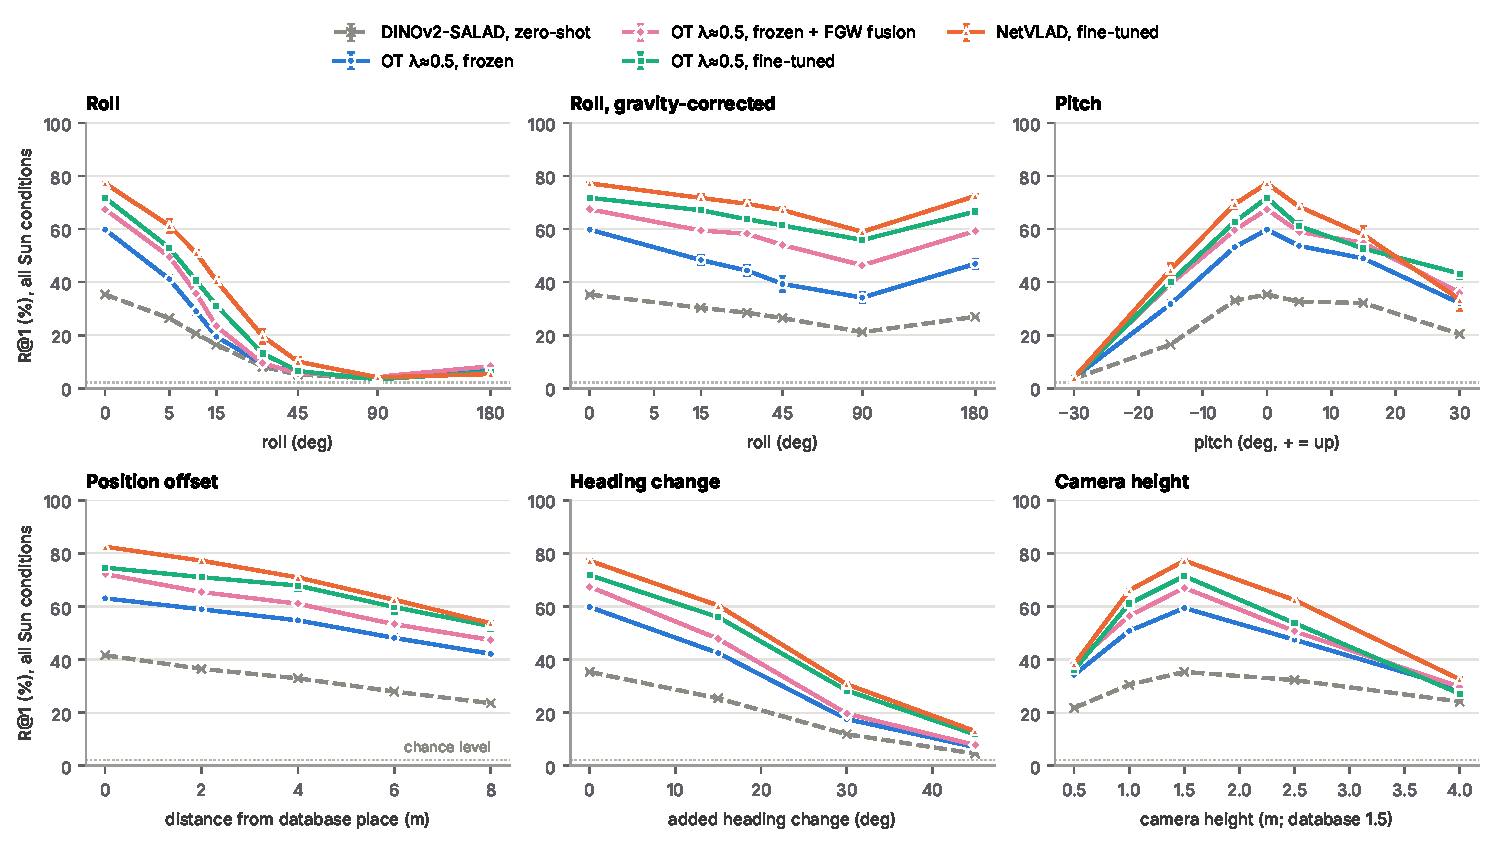
\includegraphics[width=0.92\textwidth]{figures/robustness.pdf}
\caption{Recall@1 over all seven Sun conditions when one factor of the query camera is changed (3 seeds,
error bars: std). Roll axes are square-root scaled; dotted line: chance ($2.2\%$).}
\label{fig:robust}
\end{figure*}
\begin{table*}[t]
\centering
\caption{Robustness to camera tilt and viewpoint: R@1 (\%) over all seven Sun conditions on the test set (3150 queries per row; chance $2.2\%$). Each row re-renders the benchmark queries at the benchmark poses with one factor changed; the database is the original upright one. Mean$\pm$std over 3 seeds; fusion on the frozen reference head, seed 0, with the validation-tuned $(\beta,\kappa)$ of the main paper.}
\label{tab:robust}
\footnotesize
\begin{tabular}{@{}lcccccccc@{}}
\toprule
 & Zero-shot & \multicolumn{2}{c}{Frozen backbone} & \multicolumn{2}{c}{Fine-tuned backbone} & \multicolumn{2}{c}{Frozen ref.\ head + fusion} \\
\cmidrule(lr){3-4}\cmidrule(lr){5-6}\cmidrule(l){7-8}
Variant & SALAD & OT & NetVLAD & OT & NetVLAD & FGW & MNN+MAGSAC++ \\
\midrule
Upright (baseline) & 35.3 & 59.8{\scriptsize$\pm$1.1} & 58.4{\scriptsize$\pm$0.5} & 71.8{\scriptsize$\pm$1.2} & 77.2{\scriptsize$\pm$0.5} & 67.4 & 68.2 \\
\addlinespace[2pt]
Roll $1^\circ$ & 33.0 & 56.1{\scriptsize$\pm$0.8} & 54.3{\scriptsize$\pm$0.3} & 66.6{\scriptsize$\pm$1.3} & 73.6{\scriptsize$\pm$0.7} & 61.7 & 64.6 \\
Roll $5^\circ$ & 26.4 & 41.1{\scriptsize$\pm$1.5} & 43.6{\scriptsize$\pm$0.8} & 52.9{\scriptsize$\pm$0.9} & 61.3{\scriptsize$\pm$2.6} & 49.6 & 54.9 \\
Roll $15^\circ$ & 16.5 & 19.5{\scriptsize$\pm$1.6} & 23.1{\scriptsize$\pm$0.9} & 31.2{\scriptsize$\pm$0.8} & 40.5{\scriptsize$\pm$1.4} & 23.4 & 35.5 \\
Roll $45^\circ$ & 5.2 & 6.1{\scriptsize$\pm$0.4} & 5.6{\scriptsize$\pm$0.7} & 6.5{\scriptsize$\pm$0.6} & 10.1{\scriptsize$\pm$1.7} & 5.7 & 6.8 \\
Roll $180^\circ$ & 6.9 & 7.8{\scriptsize$\pm$0.3} & 5.3{\scriptsize$\pm$0.3} & 6.1{\scriptsize$\pm$0.5} & 5.4{\scriptsize$\pm$1.1} & 8.3 & 8.2 \\
\addlinespace[2pt]
Roll $45^\circ$, gravity-corr. & 26.5 & 39.4{\scriptsize$\pm$2.9} & 39.3{\scriptsize$\pm$1.6} & 61.4{\scriptsize$\pm$1.2} & 67.2{\scriptsize$\pm$1.1} & 54.0 & 57.3 \\
Roll $180^\circ$, gravity-corr. & 26.9 & 46.9{\scriptsize$\pm$1.9} & 46.5{\scriptsize$\pm$1.2} & 66.6{\scriptsize$\pm$0.5} & 72.4{\scriptsize$\pm$0.7} & 59.3 & 63.0 \\
\addlinespace[2pt]
Pitch $-30^\circ$ & 3.7 & 4.0{\scriptsize$\pm$0.3} & 4.0{\scriptsize$\pm$0.3} & 3.8{\scriptsize$\pm$0.3} & 4.0{\scriptsize$\pm$0.5} & 4.6 & 4.7 \\
Pitch $-15^\circ$ & 16.5 & 31.7{\scriptsize$\pm$1.5} & 29.3{\scriptsize$\pm$1.5} & 40.2{\scriptsize$\pm$0.4} & 44.6{\scriptsize$\pm$2.4} & 39.4 & 43.6 \\
Pitch $+15^\circ$ & 32.2 & 49.0{\scriptsize$\pm$0.9} & 48.2{\scriptsize$\pm$0.6} & 52.7{\scriptsize$\pm$3.3} & 57.8{\scriptsize$\pm$3.2} & 54.8 & 56.9 \\
Pitch $+30^\circ$ & 20.5 & 32.1{\scriptsize$\pm$0.3} & 20.9{\scriptsize$\pm$1.4} & 43.2{\scriptsize$\pm$1.8} & 33.5{\scriptsize$\pm$4.4} & 36.0 & 42.0 \\
\addlinespace[2pt]
Offset $0$\,m & 41.6 & 63.1{\scriptsize$\pm$0.6} & 66.7{\scriptsize$\pm$0.4} & 74.6{\scriptsize$\pm$1.3} & 82.5{\scriptsize$\pm$0.3} & 72.2 & 72.8 \\
Offset $4$\,m & 32.9 & 54.8{\scriptsize$\pm$0.8} & 51.4{\scriptsize$\pm$0.4} & 67.8{\scriptsize$\pm$2.1} & 70.9{\scriptsize$\pm$0.6} & 61.0 & 62.5 \\
Offset $8$\,m & 23.6 & 42.2{\scriptsize$\pm$1.0} & 37.8{\scriptsize$\pm$0.4} & 52.6{\scriptsize$\pm$2.0} & 53.6{\scriptsize$\pm$0.9} & 47.4 & 47.6 \\
\addlinespace[2pt]
Heading $+15^\circ$ & 25.4 & 42.5{\scriptsize$\pm$1.1} & 40.0{\scriptsize$\pm$0.1} & 56.0{\scriptsize$\pm$1.1} & 60.4{\scriptsize$\pm$0.2} & 47.8 & 49.3 \\
Heading $+30^\circ$ & 11.9 & 17.6{\scriptsize$\pm$0.6} & 16.8{\scriptsize$\pm$0.4} & 28.4{\scriptsize$\pm$0.6} & 30.7{\scriptsize$\pm$0.7} & 19.6 & 20.4 \\
\addlinespace[2pt]
Height $0.5$\,m & 21.8 & 34.2{\scriptsize$\pm$0.9} & 33.0{\scriptsize$\pm$0.3} & 36.0{\scriptsize$\pm$1.7} & 38.2{\scriptsize$\pm$0.5} & 38.5 & 38.2 \\
Height $1.0$\,m & 30.5 & 50.8{\scriptsize$\pm$1.3} & 50.5{\scriptsize$\pm$1.2} & 61.1{\scriptsize$\pm$1.6} & 66.0{\scriptsize$\pm$0.4} & 56.4 & 56.6 \\
Height $2.5$\,m & 32.2 & 47.5{\scriptsize$\pm$0.5} & 48.4{\scriptsize$\pm$0.9} & 53.7{\scriptsize$\pm$1.4} & 62.4{\scriptsize$\pm$0.7} & 50.7 & 52.4 \\
Height $4.0$\,m & 24.2 & 29.0{\scriptsize$\pm$1.4} & 30.9{\scriptsize$\pm$0.6} & 27.1{\scriptsize$\pm$1.8} & 32.5{\scriptsize$\pm$0.7} & 29.7 & 29.1 \\
\bottomrule
\end{tabular}
\end{table*}

\paragraph*{Roll} Roll is the most damaging factor. A $1^\circ$ roll already costs the frozen reference head
$\rbRollOneDrop$ points (paired 95\% CI $[\rbRollOneLo,\rbRollOneHi]$), $5^\circ$ leaves $\rbRollFive\%$ and
$15^\circ$ $\rbRollFifteen\%$. From $45^\circ$ on, no model exceeds $\rbRollBigMax\%$; upside down, frozen
the reference head reaches $\rbRollUpside\%$ and fine-tuned NetVLAD $\rbFtNvRollUpside\%$. Fine-tuning does not remove the sensitivity:
fine-tuned NetVLAD falls from $\rbFtNvBase$ to $\rbFtNvRollFive\%$ at $5^\circ$. No training or database image
is rolled, and DINOv2 tokens are not rotation-invariant. Levelling the image with gravity recovers most of
the loss. Upside down, it brings the frozen reference head back to $\rbDerotGal\%$ and fine-tuned NetVLAD to
$\rbDerotFtNv\%$. The remaining cost, $\rbDerotCostGalLo$--$\rbDerotCostGalHi$ points for the frozen reference head and
$\rbDerotCostFtLo$--$\rbDerotCostFtHi$ for the fine-tuned models, comes from the black regions outside the
rolled frame.

\paragraph*{Pitch} Pitching by $\pm5^\circ$ costs the frozen reference head up to $\rbPitchFiveDrop$ points. Looking
$30^\circ$ down, the frame shows only ground within a few metres and no horizon; no model exceeds
$\rbPitchDownMax\%$. Part of this failure may be due to the simulator, whose near-field ground is limited by
the $0.3$\,m DEM. Looking $30^\circ$ up, the frame is mostly sky. The OT head then beats NetVLAD both with a
frozen backbone ($\rbPitchUpGal$ vs.\ $\rbPitchUpNv\%$) and with a fine-tuned one ($\rbPitchUpFtGal$ vs.\
$\rbPitchUpFtNv\%$). This is consistent with the dust-bin acting as a gate on sky tokens
(\cref{prop:dustbin}), although the two heads also differ in their aggregation.

\paragraph*{Viewpoint} Moving $8$\,m away from the database place costs the frozen reference head $\rbOffEightDrop$
points relative to $0$\,m. Adding $15^\circ$ or $30^\circ$ of heading costs $\rbHeadFifteenDrop$ and
$\rbHeadThirtyDrop$ points. Each place is in the database with a single heading, and most of the frame shows
nearby ground, which changes completely when the rover turns. Camera heights of $1.0$ and $2.5$\,m
(database: $1.5$\,m) cost $\rbHeightNearLo$--$\rbHeightNearHi$ points, and $0.5$ and $4.0$\,m
$\rbHeightFarLo$--$\rbHeightFarHi$.

\paragraph*{Fusion} Under small tilts and offsets, fusion still adds $\rbFusLo$--$\rbFusHi$ points. Once the
correct place leaves the ten candidates it cannot help. Under roll, MNN+MAGSAC++ fusion degrades less than
FGW ($\rbRollFifteenMnn$ vs.\ $\rbRollFifteenFgw\%$ at $15^\circ$): FGW's structural term is
rotation-invariant (\cref{prop:inv}), but its appearance term is not.

\paragraph*{Implications} A rover should level its images with the IMU before retrieval. Its database should
be recorded at the operating camera height and with several headings per place. Offsets of a few metres
cost little ($\rbOffFourDrop$ points at $4$\,m).

\end{document}
